\documentclass{article}
\usepackage[utf8]{inputenc}
\usepackage[T1]{fontenc}
\usepackage[ngerman]{babel}
\usepackage[backend=biber, style=numeric, sorting=none]{biblatex}
\usepackage{graphicx}
\usepackage{float}
\usepackage{amsmath}
\usepackage{subcaption}
\usepackage{wrapfig}
\usepackage{comment}
\usepackage[printonlyused]{acronym}
\usepackage{gensymb}
\usepackage{circuitikz}
<<<<<<< HEAD
=======
\usepackage{newfloat}
>>>>>>> 12ac912d5f0cd10c8a41cde0f36251f4203ee1ef

%\addbibresource{Vorlage.bib}
\DeclareFloatingEnvironment[
	placement=H,
	fileext=lofm,
	listname=Formelverzeichnis,
	name=Formel
]{formel}
\DeclareFloatingEnvironment[name=Schaltbild]{circuit}
\addto\captionsngerman{%
	\renewcommand{\abstractname}{Abstract}
}
\renewenvironment{abstract}{
	\begin{center}
		\normalfont\normalsize
		\bfseries \abstractname\vspace{-.5em}
	\end{center}
	\noindent
	\normalsize
}{}

\begin{document}
	\begin{titlepage}
		
		\centering
		\begin{figure}
			\centering
			
\includegraphics[width=\textwidth]{images/OTH_Logo_farbig__zweizeilig_.jpg}
		\end{figure}
		
		{\Huge \textbf{
				Versuch 1: Einphasiger Transformator\\
		}}
		\vspace{0.5cm}
		{\LARGE \textbf{
				Versuchsdurchführung am 04.05.2026\\
		}}
		\vspace{2cm}
		{\large
			Bachelorstudiengang Elektro- und Informationstechnik\\
			Fakultät Elektrotechnik, Medien und Informatik\\
			Sommersemester 2026\\
			\vspace{2cm}
		}
		
		{\large
			Gruppe B\\
			\vspace{0.3cm}
			Sebastian Eiglsperger\\
			s.eiglsperger@oth-aw.de\\
			\vspace{0.3cm}
			Lukas Maier\\
			l.maier@oth-aw.de
		}
		
		\vfill
		\thispagestyle{empty} % Diese Titelseite soll keine Seitenanzahl bekommen
		
	\end{titlepage}
	
	\setcounter{figure}{0}
	\pagenumbering{roman}
	\tableofcontents % Nur hinzufügen wenn erwünscht!
	\listoffigures
	\listoftables
	\listofformels
	\newpage	
	\section*{Abkürzungsverzeichnis}
		Test
	
	\newpage
	\pagenumbering{arabic}
	
	\section{Versuchsvorbereitung}
		Wenn nicht explizit genannt, wurde für alle Simulationen eine Messdauer von 0.0s - 10.0s, sowie eine Schrittweite von $1\cdot10^{-3}$s gesetzt.\\
<<<<<<< HEAD
		Für etwaige Messdaten Auswertungen wurde die kostenfreie MATLAB Alternative "GNU Octave" verwendet.
		\subsection{Aufbau des Simulationsmodells in PLECS}
		\label{sec:plecs_modell}
			\begin{figure}[H]
				\centering
				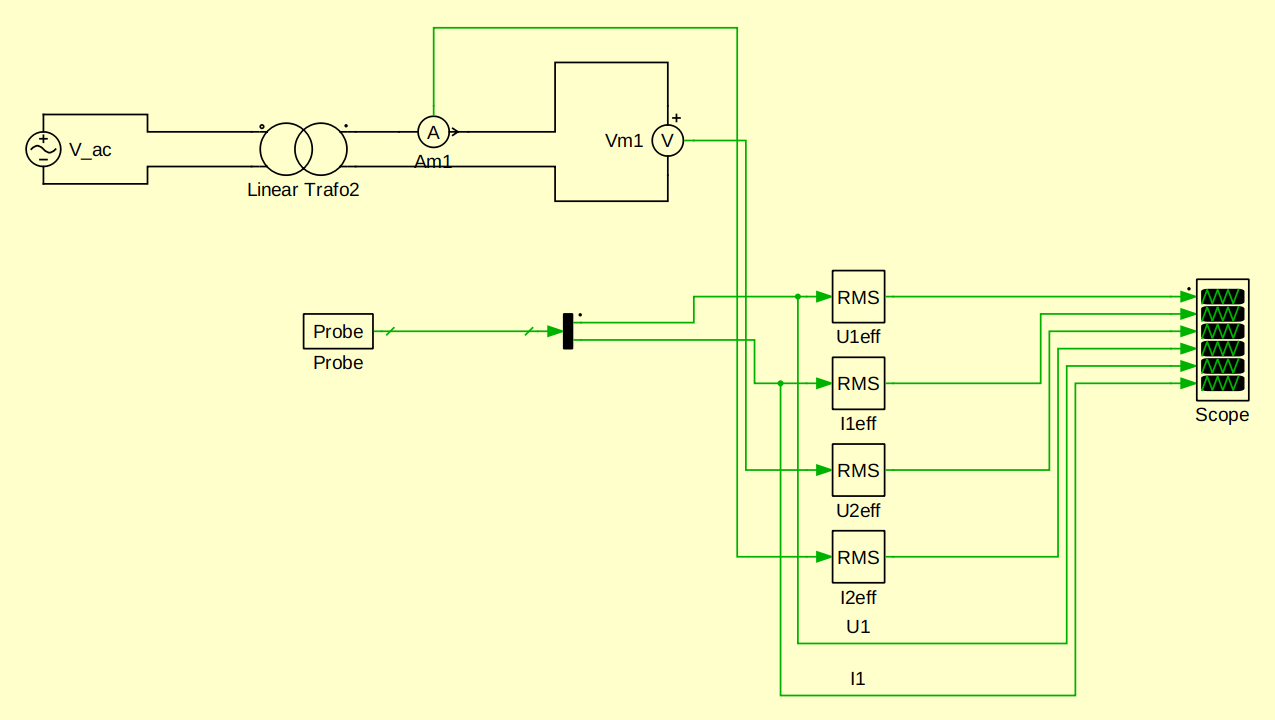
\includegraphics[width=\textwidth]{images/Vorb-1-1.png}
				\caption{Angepasster Aufbau des PLECS-Modells}
			\end{figure}
			
			Die Parameter des Modells sind der Anleitung des Versuchs entnommen:
			\begin{align*}
				U_{1, eff} &= 400V \\
				I_{2, eff} &= 20A \\
				R_1 &= 1 \Omega \\
				R_2 &= 1 \Omega \\
				L_h &= 1 H \\
				L_{1\sigma} &= 10 mH \\
				L_{2\sigma} &= 1 mH \\
				\frac{N_1}{N_2} &= 10 \\
				R_{Fe} &\rightarrow \infty
			\end{align*}
			
			Dabei ergaben sich folgende Simulationsergebnisse:
			\begin{itemize}
				\item Effektivwert der Primärspannung: 0.7V
				\item Effektivwert der Sekundärspannung: 0.7V
				\item Effektivwert des Primärstroms: 0A
				\item Effektivwert des Sekundärstroms: 0A
			\end{itemize}


		\subsection{Simulation der Leerlaufkennlinie}
			Die Primärspannung wurde von 10\% bis 110\% in 20\% Schritten variiert. 100\% stellt hierbei 230V Effektivspannung auf der Primärseite dar. An der sekundären Seite wurden lediglich ein Ampermeter und ein Voltmeter angeschlossen, um eine Sinnvolle Leerlaufkennlinie zu messen.\\
			\begin{figure}[H]
				\centering
				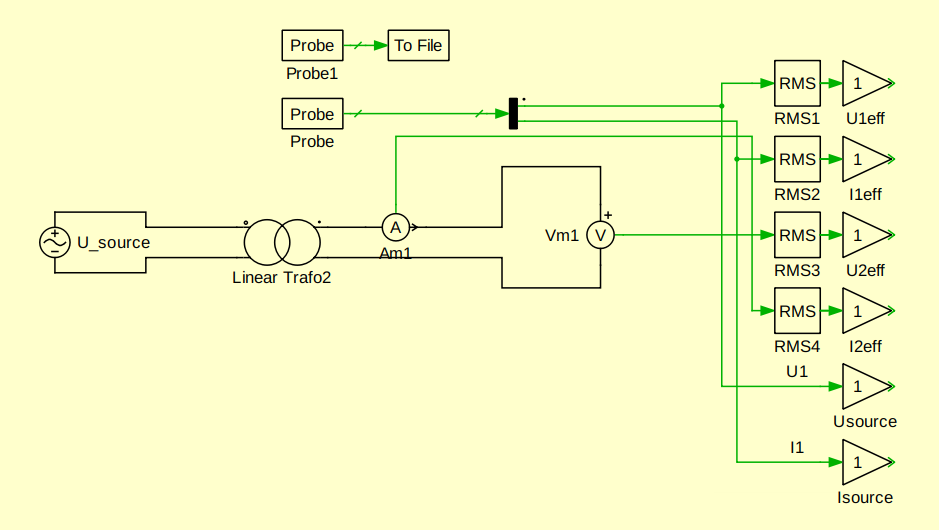
\includegraphics[width=\textwidth]{images/Vorb-1-2-Leerlauf-Aufbau.png}
				\caption{Messaufbau der Leerlaufkennliniensimulation in PLECS}
			\end{figure}
			Da die Simulationen stets bei 0.0s beginnen und der Transformator auch hier eine Einschwingzeit benötigt, wurde für die gesamten Messdaten der jeweilige Mittelwert berechnet und auch nur dieser eingezeichnet. Da die Simulationsdauer (3s) deutlich länger ist als die Einschwingdauer (ca. 0.2s) entspricht der Mittelwert der Messwerte den Werten des stationären Zustands.
			
			
			\subsubsection{Effektivwert des Leerlaufstroms $I_{10}$ über Effektivwert der Primärspannung $U_1$}
				\begin{figure}[H]
					\centering
					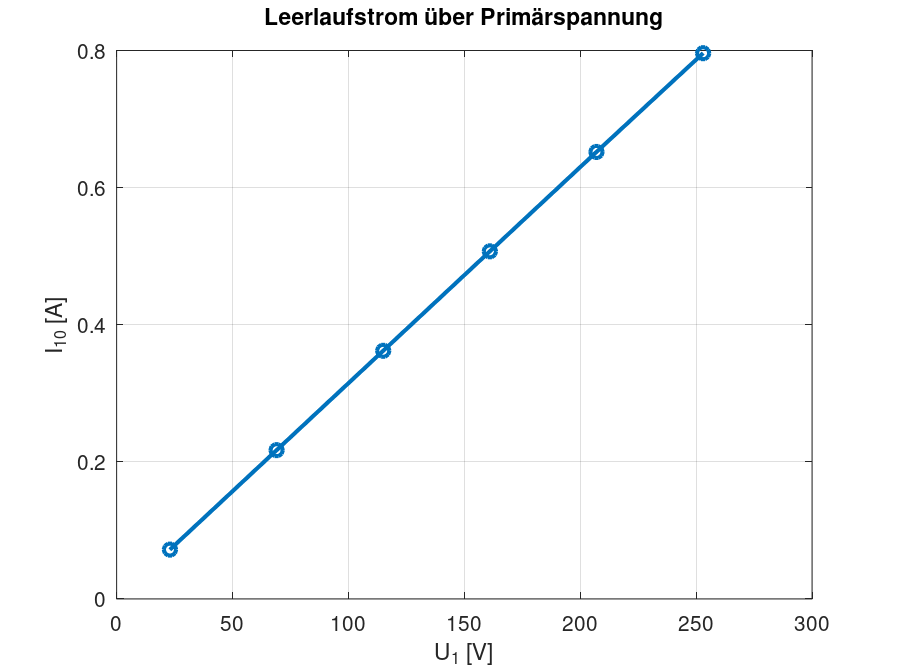
\includegraphics[width=\textwidth]{images/Vorb-1-2-Leerlauf-Leerlaufstrom.png}
					\caption{Effektivwert des Leerlaufstroms $I_{1, eff}$ über Effektivwert der Primärspannung $U_{1, eff}$}
					\label{fig:Vorb-1-2-Leerlauf_I1-U1}
				\end{figure}
				
				Zur Validierung der simulierten Messwerte wird zweckmäßigerweise das Ersatzschaltbild (ESB) des einphasigen Transformators in diesem Betriebszustand herangezogen. Im Unterschied zum im Vorlesungsskript dargestellten ESB können die Eisenverluste ($R_{FE})$ in diesem Fall vernachlässigt werden, da der entsprechende Widerstand gemäß der Parameter aus Abschnitt~\ref{sec:plecs_modell} als unendlich groß angenommen wird.
				
			\begin{circuitikz}
				% Spannungsquelle links
				\draw (0,0) to[sV, l=$U_1$] (0,3)
				
				% Serienzweig: R1 und L1σ mit Strompfeil I10
				to[R, l=$R_1$, i=$I_{10}$] (3,3)
				to[L, l=$L_{1\sigma}$] (6,3)
				
				% L1H mit äußerem Spannungspfeil
				to[L, l_=$L_{1H}$, v^=$U_{1H}$] (6,0)
				
				
				% Rückleitung
				-- (0,0);
			\end{circuitikz}
			
			Gegeben sind die Parameter der Schaltung:
			$R_1 = 1\,\Omega$, $L_{1\sigma} = 0{,}01\,\text{H}$ und $L_{1H} = 1\,\text{H}$ sowie die Frequenz $f = 50\,\text{Hz}$.
			
			Die Impedanz ergibt sich zu:
			
			\[
			\underline{Z} = R_1 + j\,2\pi f (L_{1\sigma} + L_{1H})
			\]
			
			Einsetzen der Werte liefert:
			
			\[
			\underline{Z} = 1 + j\,2\pi \cdot 50 \cdot (0{,}01 + 1)
			\]
			
			\[
			\underline{Z} = 1 + j\,2\pi \cdot 50 \cdot 1{,}01
			\]
			
			\[
			\underline{Z} \approx 1 \Omega+ j\,317{,}3 \Omega =317,3*e^{j89,82°}\,\Omega
			\]
			
			Die Admittanz ergibt sich als Kehrwert der Impedanz:
			
			\[
			\underline{Y} = \frac{1}{Z} = \frac{1}{317,3*e^{j89,82°}}=3,15 mS *e^{-j89,82°}
			\]
			
			Da im Diagramm der Strom über der Spannung aufgetragen wurde, entspricht die Steigung der Geraden dem Betrag der Admittanz.
			
			Der letzte Messpunkt hat näherungsweise die Koordinaten $U_2 = 253\,\text{V}$ und $I_2 = 0{,}8\,\text{A}$, der erste Punkt $U_1 = 23\,\text{V}$ und $I_1 = 0{,}00696\,\text{A}$.
			
			Die Steigung ergibt sich zu:
			
			\[
			m = \frac{\Delta I}{\Delta U}
			= \frac{I_2 - I_1}{U_2 - U_1}
			\]
			
			Einsetzen der Werte:
			
			\[
			m = \frac{0{,}8 - 0{,}00696}{253 - 23}
			\]
			
			\[
			m = \frac{0{,}79304}{230}
			\]
			
			\[
			m \approx 3{,}18 \cdot 10^{-3}\,\text{S}
			\]
			
			Vergleicht man den berechneten Wert mit dem aus der Simulation ermittelten Wert, so zeigt sich eine gute Übereinstimmung. Daraus lässt sich schließen, dass die Simulationsergebnisse plausibel sind und das zugrunde liegende Modell korrekt abgebildet wurde.
			
			
			\subsubsection{Effektivwert der Sekundärspannung $U_2$ über Effektivwert der Primärspannung $U_1$}
				\begin{figure}[H]
					\centering
					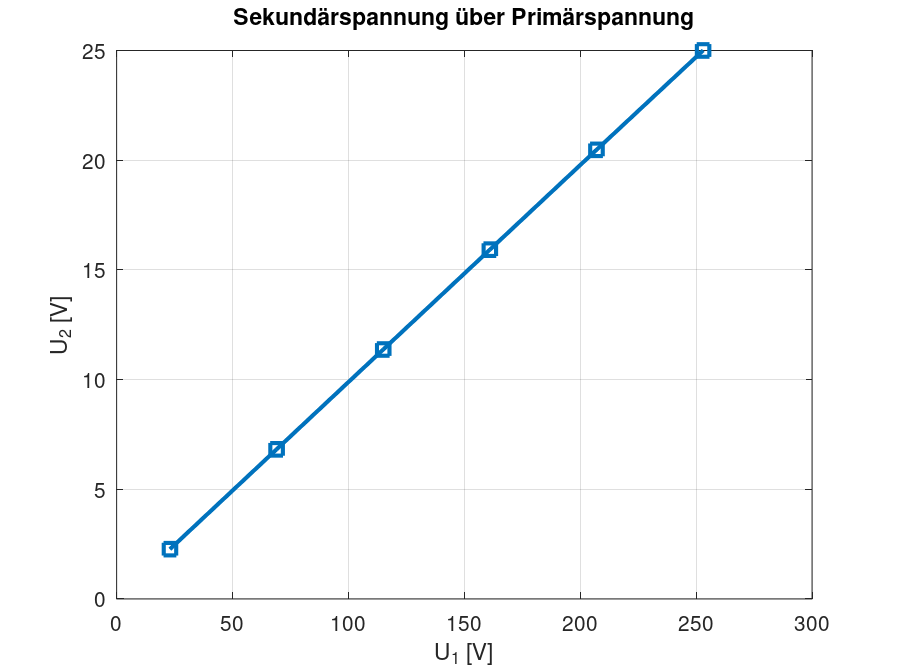
\includegraphics[width=\textwidth]{images/Vorb-1-2-Leerlauf-Sekundärspannung.png}
					\caption{Effektivwert der Sekundärspannung $U_{2}$ über Effektivwert der Primärspannung $U_{1}$}
				\end{figure}
				Die Sekundärspannung wird vorrangig durch den Windungsfaktor $"u$ mit 
				$$
				"u = \frac{N_1}{N_2} = 10
				$$
				festgelegt. \\
				
				Es folgt somit, dass $U_2$ idealerweise stets ein Zehntel der Primärspannung betragen sollte.
				
				Bei der Betrachtung des Graphen zeigt sich, dass die Simulation dieses theoretisch erwartete Verhalten sehr gut bestätigt und das entsprechende Verhältnis zwischen Primär- und Sekundärspannung korrekt abbildet.
			
			
			\subsubsection{Leistungsfaktor $cos(\varphi)$ im Leerlauf über Effektivwert der Primärspannung $U_1$}	
			
				\begin{figure}[H]
					\centering
					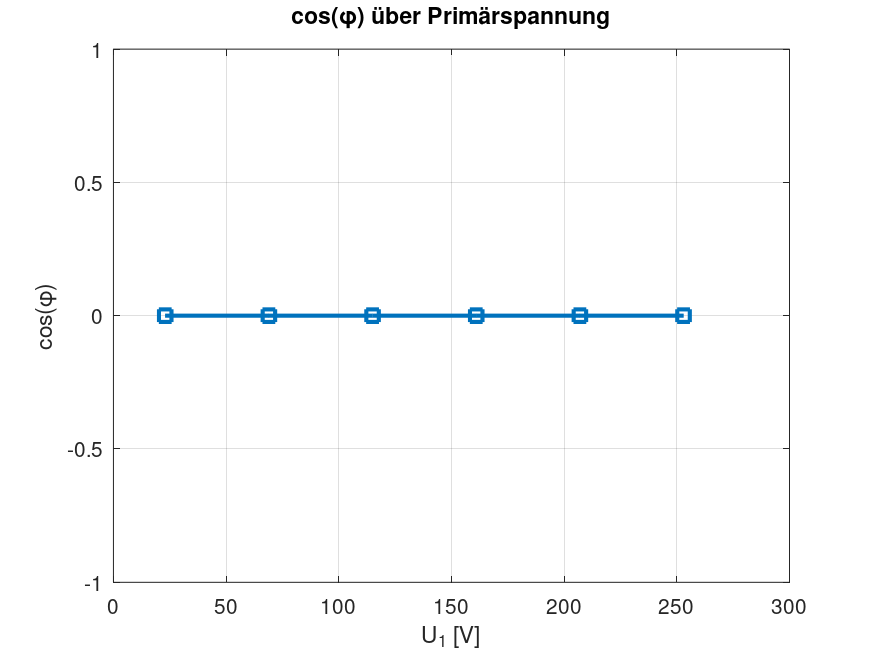
\includegraphics[width=0.7\linewidth]{images/Vorb-1-2-Leerlauf-cosphi}
					\caption{Leistungsfaktor $cos(\varphi)$ über Leerlaufspannung}
					\label{fig:vorb-1-2-leerlauf-cosphi}
				\end{figure}
				
			Zur Validierung kann man die Berechnung von $S$ über die folgende Formel heranziehen:
			
			\[
			\underline{S} = \underline{U}^2 \cdot \underline{Y^*}
			\]
			
			Nimmt man für die Spannung $\underline{U}$ einen Phasenwinkel von $0^\circ$ an, so ergibt sich der negative Phasenwinkel der Admittanz direkt als Winkel der Scheinleistung bzw. als Winkel des Leistungsfaktors.
			
			Aus den vorherigen Betrachtungen folgt für die Admittanz näherungsweise ein Winkel von etwa $-90^\circ$. Dies entspricht einem Leistungsfaktor von
			
			\[
			\cos(\varphi) \approx 0
			\]
			
			Da sich die Admittanz bei Änderungen der Spannungsamplitude nicht verändert, bleibt auch der Leistungsfaktor $\cos(\varphi)$ für alle Messpunkte konstant. Die Simulationswerte sind daher plausibel.
				
			
				
				
		\subsection{Simulation des Kurzschlusses}
			Im Simulationsmodell wird nun ein Sekundärseitiger Kurzschluss hergestellt. Die Spannung auf der Primärseite $U_1$ des Transformators wird langsam erhöht, bis der Kurzschlussstrom $I_{1k}$ ca. $100mA$ beträgt.\\
			Anschließend wird in $100mA$ Schritten bis $1A$ erhöht.
			\begin{figure}[H]
				\centering
				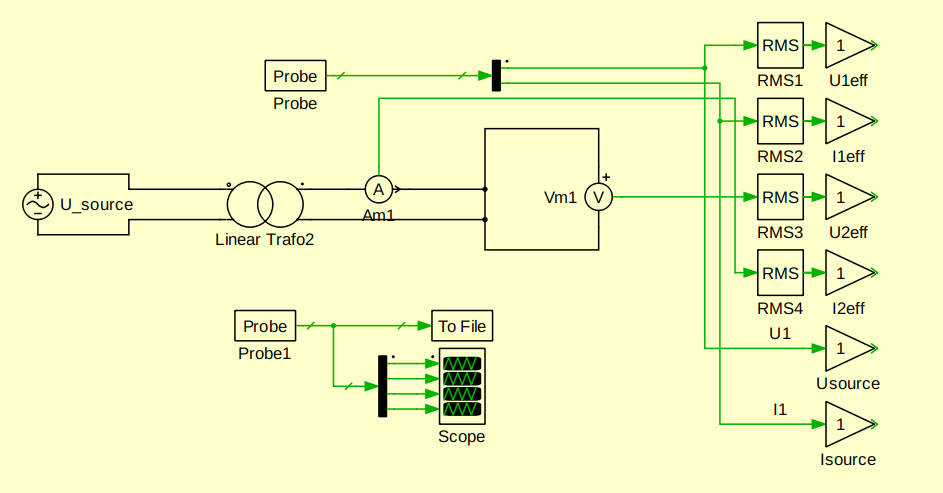
\includegraphics[width=\textwidth]{images/Vorb-1-3.png}
				\caption{Messaufbau der Kurzschlusssimulation in PLECS}
			\end{figure}
			
			Daraus ergaben sich folgende Werte:
			\begin{table}[H]
				\begin{tabular}{c|c|c|c|c|c|c|c|c|c|c}
					$U_1$ in V&  9.4 & 18.8 & 28.2 & 37.6 & 47 & 56.4 & 65.8 & 75.2 & 84.6 & 94\\
					$I_{1k}$ in A& 0.1 & 0.2 & 0.3 & 0.4 & 0.5 & 0.6 & 0.7 & 0.8 & 0.9 & 1.0\\
				\end{tabular}
			\end{table}
			
			\subsubsection{Effektivwert des Kurzschlussstroms $I_{1k}$ über Effektivwert der Primärspannung $U_1$}
				\begin{figure}[H]
					\centering
					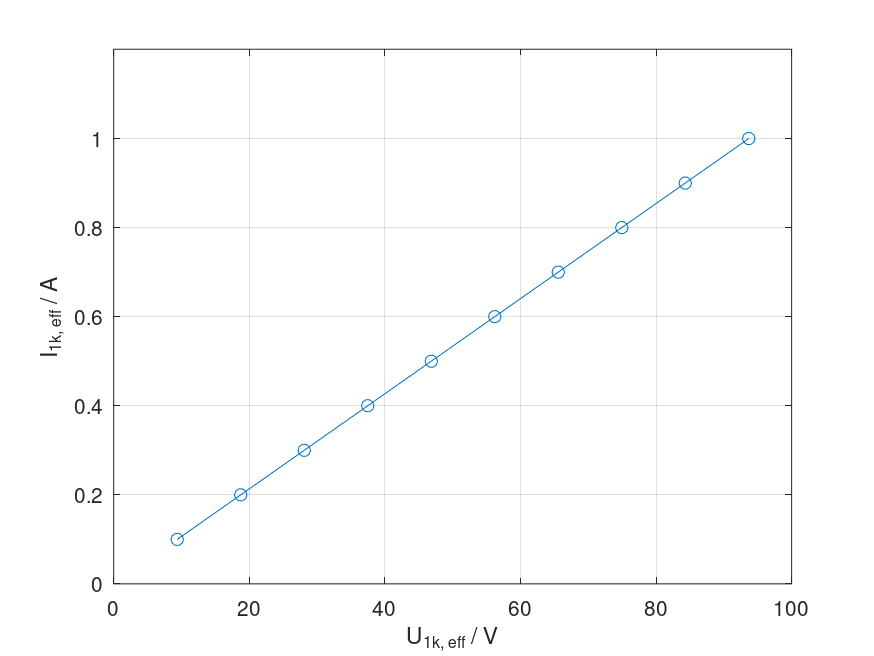
\includegraphics[width=\textwidth]{images/Vorb-1-3-Kurzschluss_I1-U1.png}
					\caption{Effektivwert des Kurzschlussstroms $I_{1k}$ über Effektivwert der Primärspannung $U_1$}
				\end{figure}
				TBC TBC TBC\\ \\
				
				Ist Linear \\
				Kurzschlussstrom $I_{1k}$ ist abhängig von $R_k$, $Z_k$ und $Z_h$.
			
			
			\subsubsection{Effektivwert des Kurzschlussstroms $I_{2k}$ über Effektivwert der Primärspannung $U_1$}
				\begin{figure}[H]
					\centering
					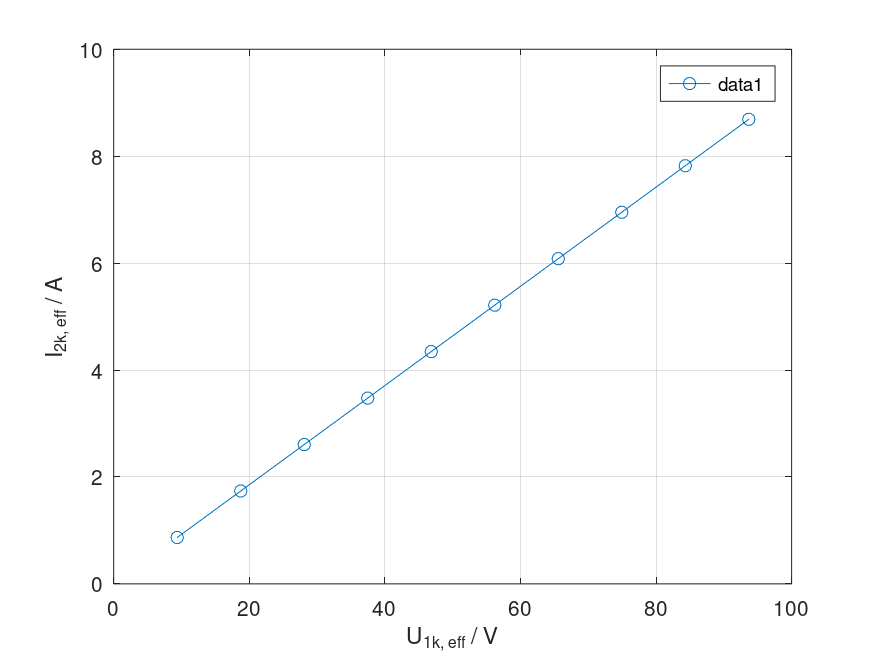
\includegraphics[width=\textwidth]{images/Vorb-1-3-Kurzschluss_I2-U1.png}
					\caption{Effektivwert des Kurzschlussstroms $I_{2k}$ über Effektivwert der Primärspannung $U_1$}
				\end{figure}
				TBC TBC TBC\\ \\
				
				Ist Linear \\
				Kurzschlussstrom $I_{2k}$ ist abhängig von $R_k$, $Z_k$, $Z_h$ und $I_{1k}$.
				
			\subsubsection{Leistungsfaktor $cos \varphi_k$ im Kurzschluss über Effektivwert der Primärspannung $U_1$}
				\begin{figure}[H]
					\centering
					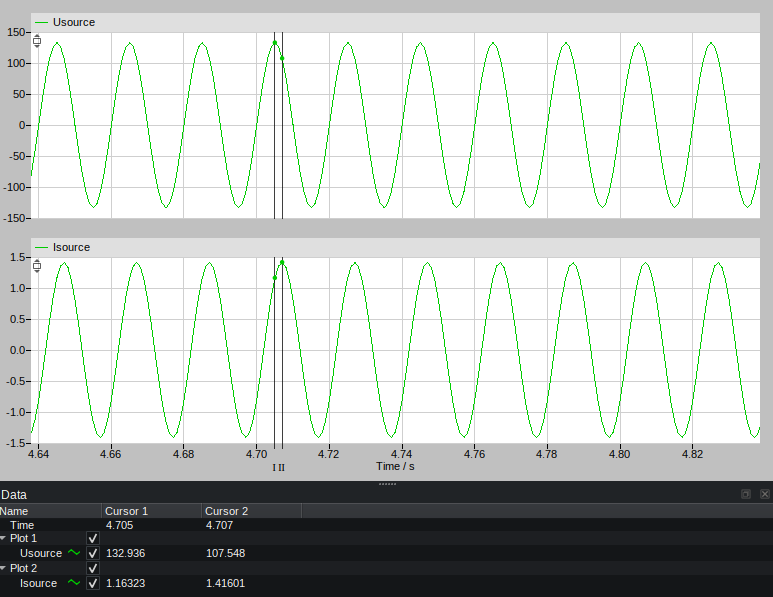
\includegraphics[width=\textwidth]{images/Vorb-1-3-Kurzschluss-Leistungsfaktor.png}
					\caption{Leistungsfaktor $cos \varphi_k$ im Kurzschluss über Effektivwert der Primärspannung $U_1$}
				\end{figure}
				Bei näherer Betrachtung ergibt $\Delta t$ einen Wert von 0.002s.\\
				Daraus folgt:
				$$
				\varphi_{UI} = 360 \cdot 50Hz \cdot 0.002s = 36\degree
				$$
				und
				$$
				cos \varphi_{UI} = 0.809
				$$
				TBC TBC TBC \\ \\
				
				Damit sich cos phi ändert, muss ich ja Impedanz ändern. Nicht Spannung oder Strom. Also bleibt cos phi auch bei allen Stufen gleich
			
		\subsection{Simulation des Einschaltstroms (Eng.: inrush current)}
			
		\begin{figure}[H]
			\centering
			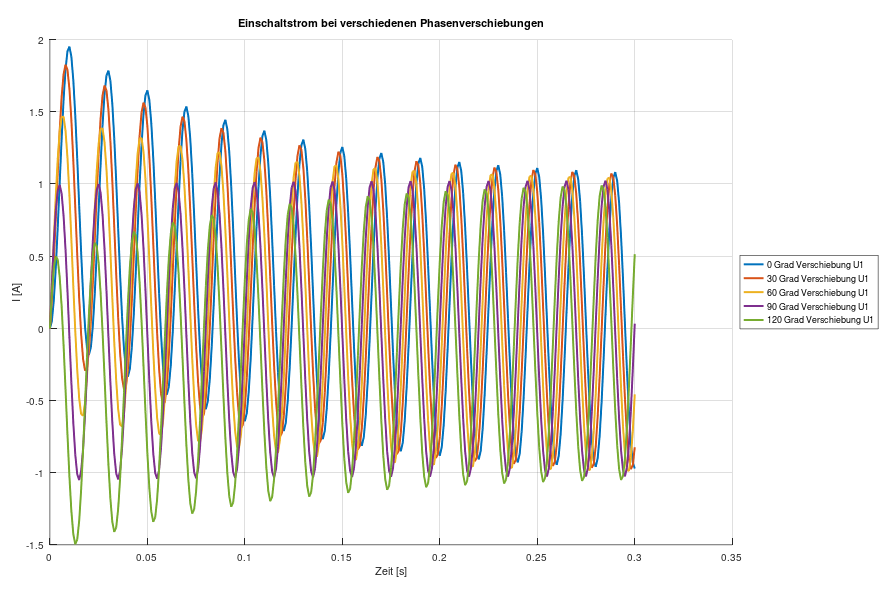
\includegraphics[width=1\linewidth]{images/Vorb-1-4-einschaltstrom}
			\caption{Einschaltstrom I1 bei verschiedenen Phasenlagen von U}
			\label{fig:vorb-1-4-einschaltstrom}
		\end{figure}
		 
=======
		Für etwaige Messdaten Auswertungen wurde die kostenfreie MATLAB Alternative "GNU Octave" verwendet. \\
		
		Ein Strang des einphasigen Transformators lässt sich gemäß Abbildung~\ref{fig:Vorb-ESBTransformator} darstellen.\\
>>>>>>> 12ac912d5f0cd10c8a41cde0f36251f4203ee1ef

		\begin{circuit}[H]
			\centering
			\begin{circuitikz}
				
				% obere Leitung
				\draw
				(0,0) node[ocirc] {}
				to[R=$R_1$, i>^=$I_1$] (3,0)
				to[L=$X_{1\sigma}$] (5,0)
				-- (6,0)
				to[L=$X'_{2\sigma}$] (9,0)
				to[R=$R'_2$, i>^=$I'_2$] (11,0)
				-- (12,0) node[ocirc] {};
				
				% untere Leitung
				\draw (0,-2) node[ocirc] {} -- (12,-2) node[ocirc] {};
				
				% linke Spannung nach unten
				\draw[->] (0,-0.2) -- (0,-1.8) node[midway, right]{$U_1$};
				
				% rechte Spannung nach unten
				\draw[->] (12,-0.2) -- (12,-1.8) node[midway, left]{$U_2'$};
				
				% Parallelzweig: X_h und R_Fe nebeneinander
				\draw (6,0) -- (6.5,0);
				\draw (6.5,0)
				to[L=$X_h$] (6.5,-2);
				
				\draw (6,0) -- (5.5,0);
				\draw (5.2,0)
				to[R=$R_{Fe}$] (5.2,-2);
				
				% Verbindung unten zur Masseleitung
				\draw (6.5,-2) -- (5.5,-2);
				
				% Magnetisierungsstrom
				\draw[->] (7.5,-0.5) -- (7.5,-1.5) node[midway,right] {$I_\mu$};
				
			\end{circuitikz}
			\caption{Ersatzschaltbild des Stranges eines einphasigen Transformators}
			\label{fig:Vorb-ESBTransformator}
		\end{circuit}
		
			\subsection{Aufbau des Simulationsmodells in PLECS}
			\label{sec:plecs_modell}
				\begin{figure}[H]
					\centering
					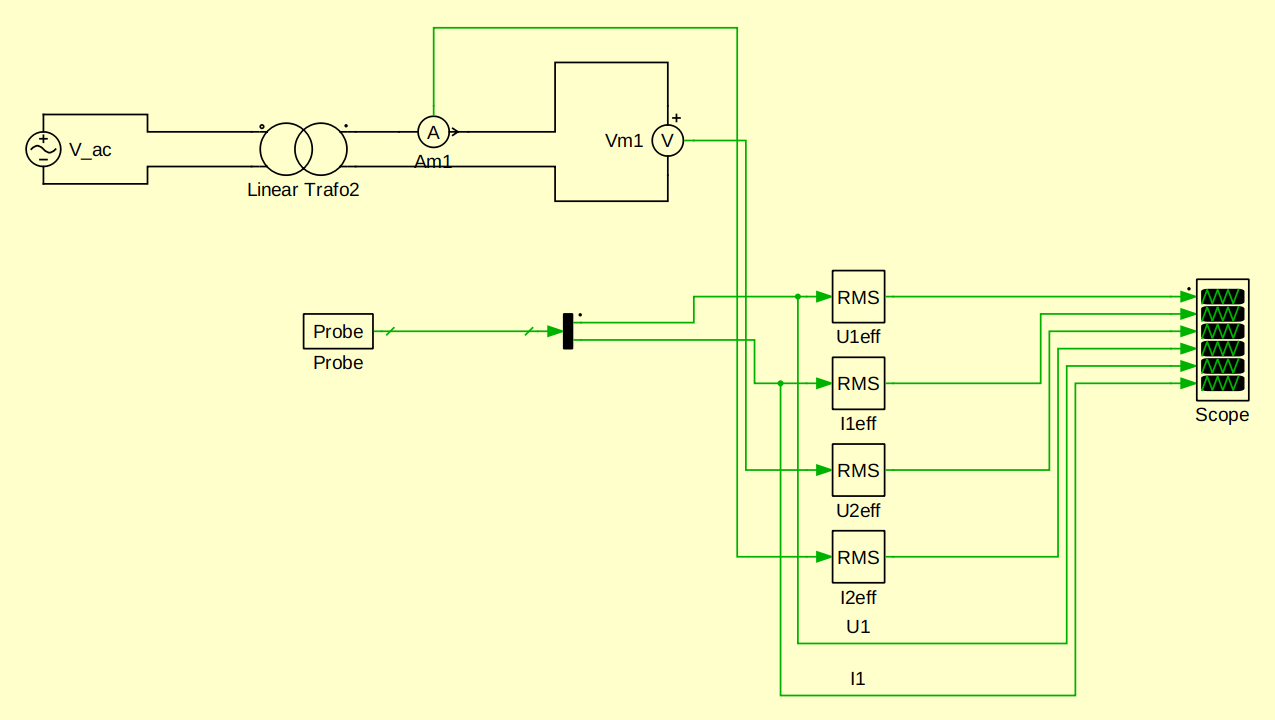
\includegraphics[width=\textwidth]{images/Vorb-1-1.png}
					\caption{Angepasster Aufbau des PLECS-Modells}
				\end{figure}
				
				Die Parameter des Modells sind der Anleitung des Versuchs entnommen:
				\begin{align*}
					U_{1, eff} &= 400V \\
					I_{2, eff} &= 20A \\
					R_1 &= 1 \Omega \\
					R_2 &= 1 \Omega \\
					L_h &= 1 H \\
					L_{1\sigma} &= 10 mH \\
					L_{2\sigma} &= 1 mH \\
					\frac{N_1}{N_2} &= 10 \\
					R_{Fe} &\rightarrow \infty
				\end{align*}
				
				Dabei ergaben sich folgende Simulationsergebnisse:
				\begin{itemize}
					\item Effektivwert der Primärspannung: 0.7V
					\item Effektivwert der Sekundärspannung: 0.7V
					\item Effektivwert des Primärstroms: 0A
					\item Effektivwert des Sekundärstroms: 0A
				\end{itemize}
	
<<<<<<< HEAD
	\subsection{2.3 Leerlauf - Messung der Leerlaufkennlinie}
	
	\begin{figure}[H]
		\centering
		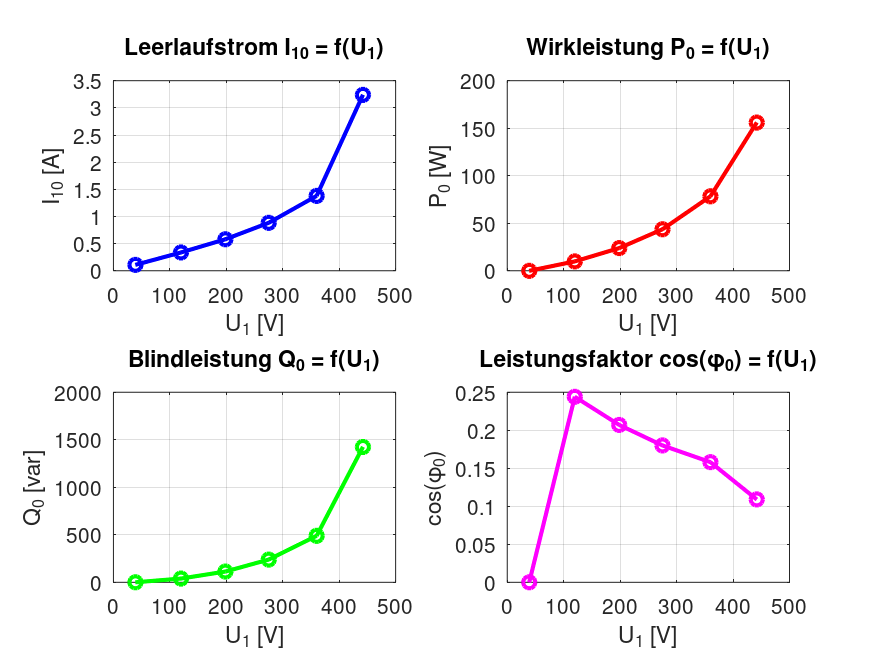
\includegraphics[width=1\linewidth]{images/durch-2-3-Leerlaufkennlinie}
		\caption{Leerlaufkennlinie des Leerlaufstroms $I_{10}$, des Leistungsfaktors $cos(\phi_{0})$, der Blindleistung $Q_0$ und der Wirkleistung $P_0$}
		\label{fig:durch-2-3-leerlaufkennlinie}
	\end{figure}
	
	\begin{table}[h!]
		\centering
		\begin{tabular}{c|c|c|c|c}
			\textbf{$U_1$ (V)} & \textbf{$I_{10}$ (A)} & \textbf{$\cos(\varphi_0)$} & \textbf{$P_0$ (W)} & \textbf{$Q_0$ (var)} \\
			\hline
			39.04  & 0.11  & 0.000 & 0.0   & 0.0   \\
			119.7  & 0.338 & 0.244 & 9.89  & 39.26 \\
			198.4  & 0.581 & 0.207 & 23.9  & 113.0 \\
			275.1  & 0.884 & 0.180 & 43.7  & 239   \\
			360    & 1.38  & 0.158 & 78.4  & 489   \\
			442    & 3.24  & 0.109 & 156   & 1424  \\
		\end{tabular}
		\caption{Messwerte des Leerlaufstroms $I_{10}$, des Leistungsfaktors $cos(\phi_{0})$, der Blindleistung $Q_0$ und der Wirkleistung $P_0$}

	\end{table}
	
	Betrachtet man den Leerlaufstrom $I_{10}$ so fällt auf das dieser im Rahmen der Mess- und Zeichenungenauigkeit bis zum Wert bei $U_1 = 360 V$ linear verläuft. Der folgende Wert bei $U_1 = 442 V$ passt nicht mehr zum linearen Verlauf. Bei Betrachtung der Wirk- und Blindleistung und den daraus resultierenden Leistungsfaktor $\cos(\varphi_0)$ fällt auf das mit steigender Spannung die Wirk- und Blindleistung steigt. Jedoch mit Zunehmenden Spannungswert von $U_1$ die Blindleistung stärker ansteigt als die Wirkleistung und in folge dessen der Leistungsfaktor des Transformators sinkt.
	
	Der erste Wert in den Messreihen ist nicht zu beachten, da dass Messgerät in diesem Messpunkt falsche Werte angezeigt hat, da zero current blocking aktiviert war.
	
	\paragraph{Diskussion der Messergebnisse}
	
	Im Leerlauf gilt näherungsweise, dass die induzierte Spannung \(U_i\) der angelegten Spannung \(U_1\) entspricht. Die magnetische Feldstärke \(H\) ist proportional zum Magnetisierungsstrom:
	
	\[
	H = \frac{NI}{l}
	\]
	
	\begin{figure}[H]
		\centering
		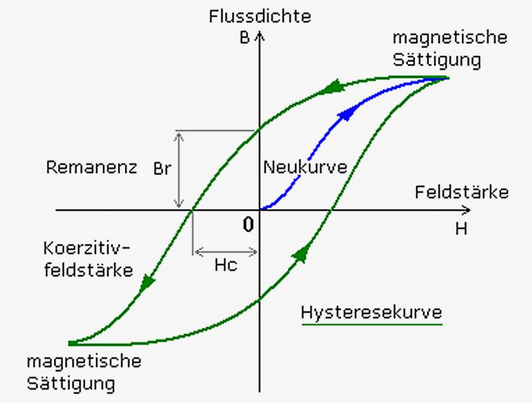
\includegraphics[width=0.7\linewidth]{images/B-H-Kennlinie}
		\caption{B-H Kennlinie\newline (Quelle: https://www.magna-c.com/lexikon/B/B-H-Kurve)}
		\label{fig:b-h-kennlinie}
	\end{figure}
	
	
	Steigt der Strom \(I\), so steigt ebenfalls die magnetische Feldstärke \(H\). Diese erzeugt im Eisenkern die magnetische Flussdichte \(B\). Im linearen Bereich der \(B\)-\(H\)-Kennlinie führt eine Erhöhung von \(H\) zu einer annähernd proportionalen Erhöhung von \(B\) (siehe Abbildung ~12). Der Zusammenhang lautet:
	
	\[
	B = \mu_r \mu_0 H
	\]
	
	Die induzierte Spannung ergibt sich aus der zeitlichen Änderung der magnetischen Flussdichte:
	
	\[
	U_i = -N A \frac{dB}{dt}
	\]
	
	Da Windungszahl \(N\) und Kernquerschnitt \(A\) konstant sind, muss bei steigender angelegter Spannung auch die Flussdichte \(B\) beziehungsweise deren zeitliche Änderung zunehmen.
	
	Bei kleinen Spannungen befindet sich der Transformator noch im linearen Bereich der Magnetisierungskennlinie, weshalb der Leerlaufstrom zunächst annähernd linear ansteigt. Ab einer Spannung von etwa \(U_1 = 442\,\mathrm{V}\) gerät der Eisenkern jedoch zunehmend in magnetische Sättigung, d.H. die Steigung im B-H Graph nimmt ab und damit entsprechend auch \(\mu_r\).
	
	Mit zunehmender Sättigung sind bereits viele Elementarmagnete des Eisenkerns ausgerichtet. Dadurch kann sich das Material nur noch geringfügig weiter magnetisieren. Die relative Permeabilität \(\mu_r\) sinkt deshalb stark ab. Folglich führt eine starke Erhöhung der magnetischen Feldstärke \(H\) nur noch zu einer kleinen Erhöhung der Flussdichte \(B\).
	
	Dadurch steigt die induzierte Gegenspannung nicht mehr proportional zur angelegten Spannung an. Die verbleibende Spannungsdifferenz verursacht einen starken Anstieg des Magnetisierungsstromes \(I_{10}\). Gleichzeitig wird mehr Energie zum Aufbau des Magnetfeldes benötigt, wodurch insbesondere die Blindleistung stark ansteigt. Da die Blindleistung stärker zunimmt als die Wirkleistung, sinkt der Leistungsfaktor \(\cos(\varphi_0)\) des Transformators.
	
	\subsection{Leerlauf - Induzierte Spannungen bei Leerlauf}
	
	\begin{table}[h]
		\centering
		\begin{tabular}{|c|c|}
			\hline
			Messgröße & Wert \\ 
			\hline
			\(U_{1U}\)   & \(401{,}6\,\mathrm{V}\) \\ 
			\hline
			\(U_{2U}\) & \(66{,}1\,\mathrm{V}\) \\ 
			\hline
			\(U_{2V}\) & \(62{,}4\,\mathrm{V}\) \\ 
			\hline
			\(U_{2W}\) & \(4{,}52\,\mathrm{V}\) \\ 
			\hline
		\end{tabular}
		\caption{Gemessene effektive Primär- und Sekundärspannungen}
		\label{tab:spannungen}
	\end{table}
	
	Bei der Messung der Sekundärspannungen des Transformators im Leerlauf fällt auf, dass die Spannungen \(U_{2U}\) und \(U_{2V}\) annähernd gleich groß sind, während die Spannung \(U_{2W}\) deutlich kleiner ausfällt. 
	
	

	\paragraph{Diskussion der Messwerte}
	
	\begin{figure}[H]
		\centering
		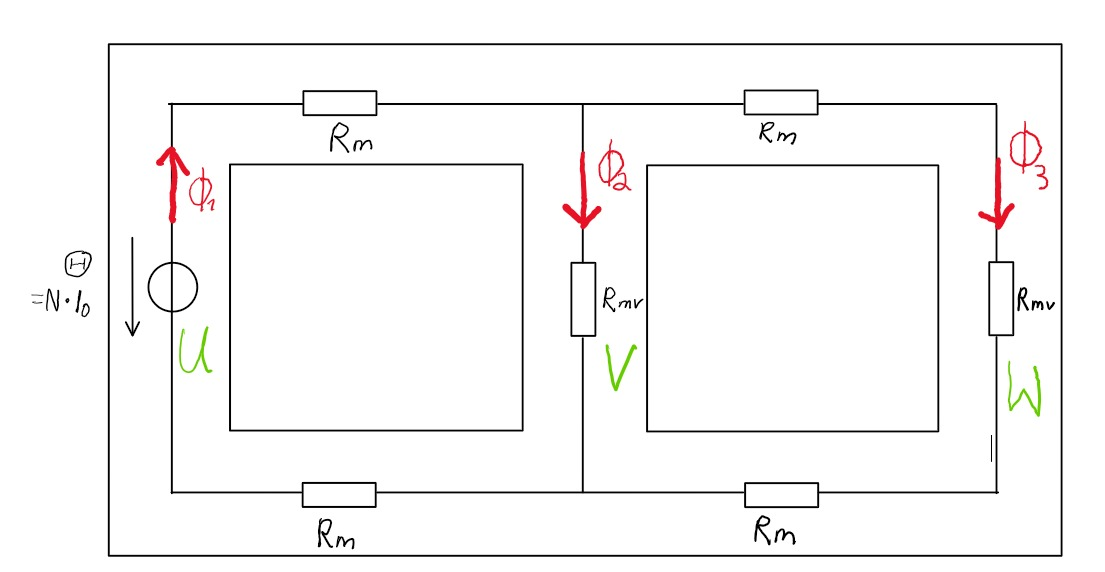
\includegraphics[width=0.7\linewidth]{images/Durch-2-4-magnetischer-Kreis}
		\caption{vereinfachter magnetischer Kreis des Transformators}
		\label{fig:durch-2-4-magnetischer-kreis}
	\end{figure}
	
Es lässt sich zeigen, dass der magnetische Fluss maßgeblich die induzierte Spannung bestimmt. Für einen vereinfachten homogenen magnetischen Kreis gilt:

\[
B = \frac{\Phi}{A}
\]

Da im linken Eisenkern die Spulen \(1U1-1U2\) und \(2U1-2U2\) übereinander angeordnet sind, wird die Spule \(2U1-2U2\) durch den größten magnetischen Fluss \(\Phi_1\) durchflossen.

Im mittleren Eisenkern teilt sich dieser Fluss auf:

\[
\Phi_1 = \Phi_2 + \Phi_3
\]

Unter der Annahme eines homogenen Materials ist der magnetische Widerstand im Zweig von \(\Phi_3\) deutlich größer (mindestens etwa dreifach) als im mittleren Eisenkern. Dadurch ist der magnetische Fluss \(\Phi_3\) entsprechend kleiner als \(\Phi_2\).

Nach dem Induktionsgesetz gilt bei Annahme eines homogenen magnetischen Kreises:

\begin{align*}
	u_i &= -N \cdot \frac{dB}{dt} \\
	u_i &= -\frac{N}{A} \cdot \frac{d\Phi}{dt} \quad
\end{align*}

Damit ist die induzierte Spannung proportional zur zeitlichen Änderung des magnetischen Flusses:

\[
U_{2U} \propto \frac{d\Phi_1}{dt}, \quad
U_{2V} \propto \frac{d\Phi_2}{dt}, \quad
U_{2W} \propto \frac{d\Phi_3}{dt}
\]

Aus der Knotenpunktregel des magnetischen Kreises folgt direkt:

\[
\frac{d\Phi_1}{dt} = \frac{d\Phi_2}{dt} + \frac{d\Phi_3}{dt}
\;\;\Rightarrow\;\;
U_{2U} = U_{2V} + U_{2W}
\]

Diese Beziehung stimmt im Rahmen der Messungenauigkeit mit den experimentellen Werten überein:



\[
66{,}1\,\text{V} \approx 62{,}4\,\text{V} + 4{,}52\,\text{V}
\]
	
\subsection{Leerlauf - Induziert Spannungen bei Leerlauf}

\begin{table}[h]
	\centering
	\begin{tabular}{|c|c|}
		\hline
		Größe & Spannung [V] \\
		\hline
		$U_{1V}$   & 397.5 \\
		$U_{2U}$ & 32.3 \\
		$U_{2V}$ & 65.4 \\
		$U_{2W}$ & 32.9 \\
		\hline
	\end{tabular}
	\caption{Primär- und Sekundärspannungen des Transformators}
\end{table}

Bei Versorgung der Spule \(1V1 - 1V2\) fällt auf, dass die Spannung \(U_{2V}\) in etwa der Summe der Spannungen \(U_{2U}\) und \(U_{2W}\) entspricht.

\paragraph{Diskussion der Messwerte}

Aus dem magnetischen Kreis in Abbildung 13 lässt sich erkennen, dass sich bei Vertauschen des mittleren magnetischen Widerstands mit der magnetischen Spannungsquelle im linken Joch der magnetische Fluss \(\Phi_2\) symmetrisch in \(\Phi_1\) und \(\Phi_3\) aufteilen muss.

Daraus folgt in Analogie zu Abschnitt 2.4, dass auch die gemessenen Spannungen dem theoretischen Verhalten entsprechen. Es gilt näherungsweise:

\[
U_{2V} \approx U_{2U} + U_{2W}
\]

Die Messwerte bestätigen somit das erwartete Verhalten des magnetischen Kreises innerhalb der Messunsicherheit.

	
=======
	
			\subsection{Simulation der Leerlaufkennlinie}
				Die Primärspannung wurde von 10\% bis 110\% in 20\% Schritten variiert. 100\% stellt hierbei 230V Effektivspannung auf der Primärseite dar. An der sekundären Seite wurden lediglich ein Ampermeter und ein Voltmeter angeschlossen, um eine Sinnvolle Leerlaufkennlinie zu messen.\\
				\begin{figure}[H]
					\centering
					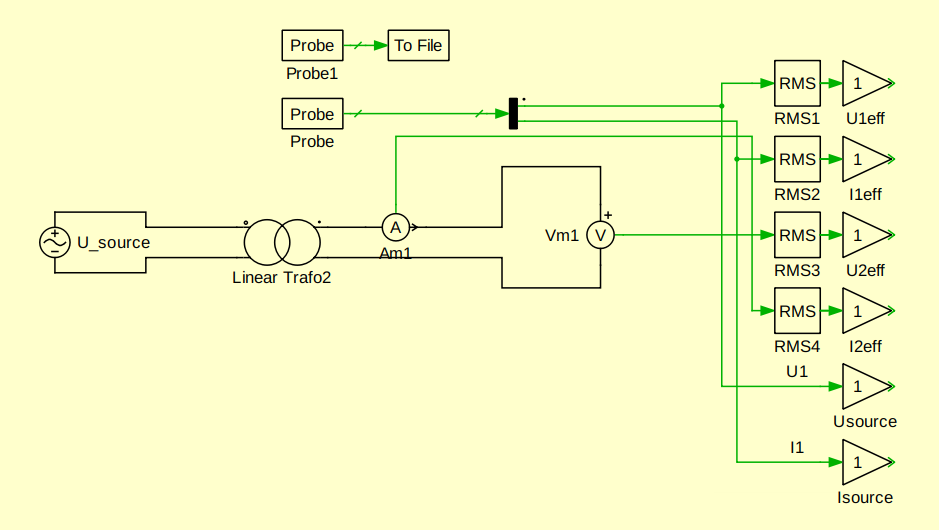
\includegraphics[width=\textwidth]{images/Vorb-1-2-Leerlauf-Aufbau.png}
					\caption{Messaufbau der Leerlaufkennliniensimulation in PLECS}
				\end{figure}
				Da die Simulationen stets bei 0.0s beginnen und der Transformator auch hier eine Einschwingzeit benötigt, wurde für die gesamten Messdaten der jeweilige Mittelwert berechnet und auch nur dieser eingezeichnet. Da die Simulationsdauer (3s) deutlich länger ist als die Einschwingdauer (ca. 0.2s) entspricht der Mittelwert der Messwerte den Werten des stationären Zustands.
				
				
				\subsubsection{Effektivwert des Leerlaufstroms $I_{10}$ über Effektivwert der Primärspannung $U_1$}
					\begin{figure}[H]
						\centering
						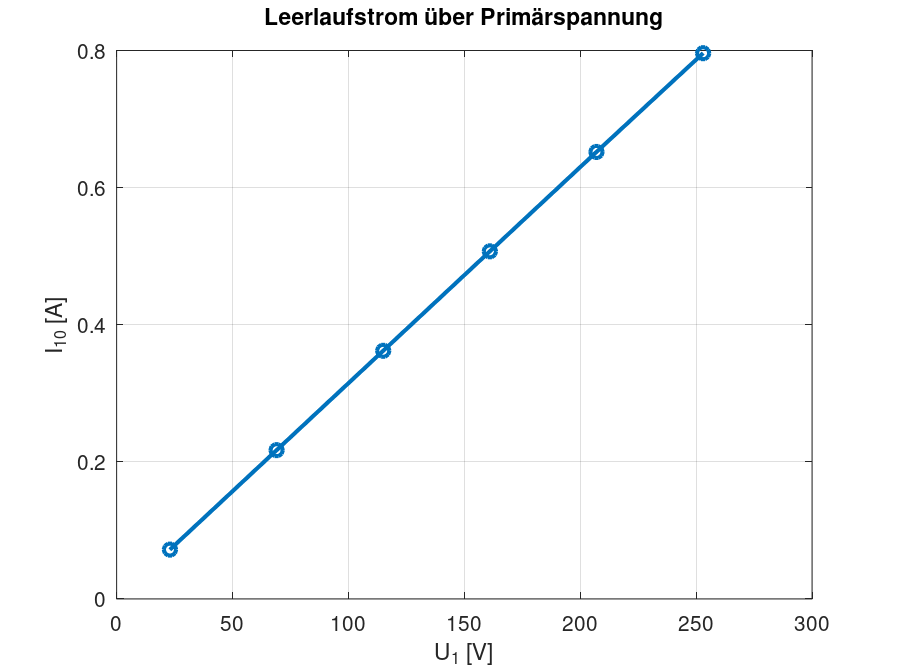
\includegraphics[width=\textwidth]{images/Vorb-1-2-Leerlauf-Leerlaufstrom.png}
						\caption{Effektivwert des Leerlaufstroms $I_{1, eff}$ über Effektivwert der Primärspannung $U_{1, eff}$}
						\label{fig:Vorb-1-2-Leerlauf_I1-U1}
					\end{figure}
					
					Zur Validierung der simulierten Messwerte wird zweckmäßigerweise das Ersatzschaltbild (ESB) des einphasigen Transformators in diesem Betriebszustand herangezogen. Im Unterschied zum im Vorlesungsskript dargestellten ESB können die Eisenverluste ($R_{FE})$ in diesem Fall vernachlässigt werden, da der entsprechende Widerstand gemäß der Parameter aus Abschnitt~\ref{sec:plecs_modell} als unendlich groß angenommen wird.
					
				\begin{circuitikz}
					% Spannungsquelle links
					\draw (0,0) to[sV, l=$U_1$] (0,3)
					
					% Serienzweig: R1 und L1σ mit Strompfeil I10
					to[R, l=$R_1$, i=$I_{10}$] (3,3)
					to[L, l=$L_{1\sigma}$] (6,3)
					
					% L1H mit äußerem Spannungspfeil
					to[L, l_=$L_{1H}$, v^=$U_{1H}$] (6,0)
					
					
					% Rückleitung
					-- (0,0);
				\end{circuitikz}
				
				Gegeben sind die Parameter der Schaltung:
				$R_1 = 1\,\Omega$, $L_{1\sigma} = 0{,}01\,\text{H}$ und $L_{1H} = 1\,\text{H}$ sowie die Frequenz $f = 50\,\text{Hz}$.
				
				Die Impedanz ergibt sich zu:
				
				\[
				\underline{Z} = R_1 + j\,2\pi f (L_{1\sigma} + L_{1H})
				\]
				
				Einsetzen der Werte liefert:
				
				\[
				\underline{Z} = 1 + j\,2\pi \cdot 50 \cdot (0{,}01 + 1)
				\]
				
				\[
				\underline{Z} = 1 + j\,2\pi \cdot 50 \cdot 1{,}01
				\]
				
				\[
				\underline{Z} \approx 1 \Omega+ j\,317{,}3 \Omega =317,3*e^{j89,82°}\,\Omega
				\]
				
				Die Admittanz ergibt sich als Kehrwert der Impedanz:
				
				\[
				\underline{Y} = \frac{1}{Z} = \frac{1}{317,3*e^{j89,82°}}=3,15 mS *e^{-j89,82°}
				\]
				
				Da im Diagramm der Strom über der Spannung aufgetragen wurde, entspricht die Steigung der Geraden dem Betrag der Admittanz.
				
				Der letzte Messpunkt hat näherungsweise die Koordinaten $U_2 = 253\,\text{V}$ und $I_2 = 0{,}8\,\text{A}$, der erste Punkt $U_1 = 23\,\text{V}$ und $I_1 = 0{,}00696\,\text{A}$.
				
				Die Steigung ergibt sich zu:
				
				\[
				m = \frac{\Delta I}{\Delta U}
				= \frac{I_2 - I_1}{U_2 - U_1}
				\]
				
				Einsetzen der Werte:
				
				\[
				m = \frac{0{,}8 - 0{,}00696}{253 - 23}
				\]
				
				\[
				m = \frac{0{,}79304}{230}
				\]
				
				\[
				m \approx 3{,}18 \cdot 10^{-3}\,\text{S}
				\]
				
				Vergleicht man den berechneten Wert mit dem aus der Simulation ermittelten Wert, so zeigt sich eine gute Übereinstimmung. Daraus lässt sich schließen, dass die Simulationsergebnisse plausibel sind und das zugrunde liegende Modell korrekt abgebildet wurde.
				
				
				\subsubsection{Effektivwert der Sekundärspannung $U_2$ über Effektivwert der Primärspannung $U_1$}
					\begin{figure}[H]
						\centering
						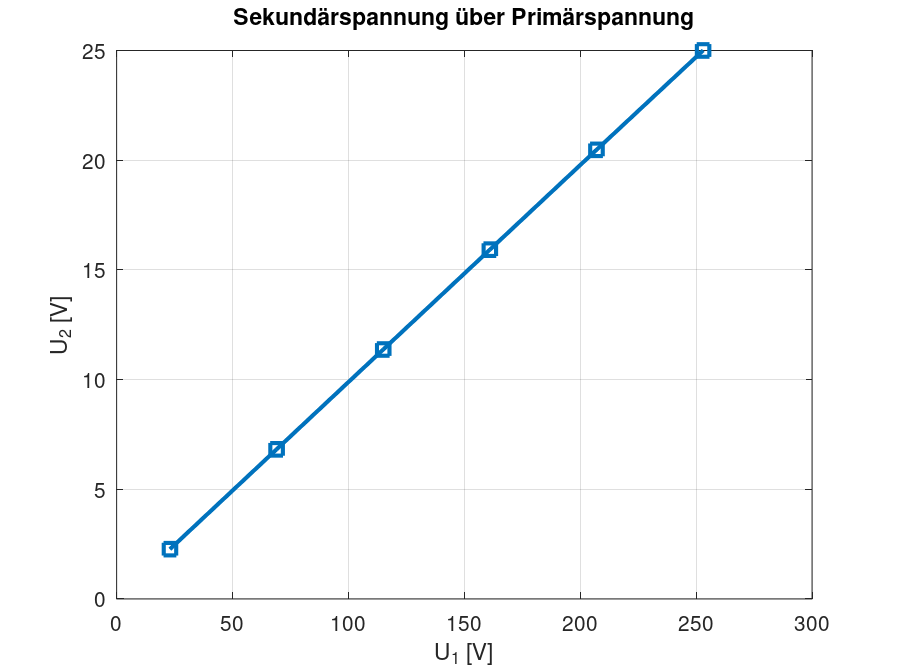
\includegraphics[width=\textwidth]{images/Vorb-1-2-Leerlauf-Sekundärspannung.png}
						\caption{Effektivwert der Sekundärspannung $U_{2}$ über Effektivwert der Primärspannung $U_{1}$}
					\end{figure}
					Die Sekundärspannung wird vorrangig durch den Windungsfaktor $"u$ mit 
					$$
					"u = \frac{N_1}{N_2} = 10
					$$
					festgelegt. \\
					
					Es folgt somit, dass $U_2$ idealerweise stets ein Zehntel der Primärspannung betragen sollte.
					
					Bei der Betrachtung des Graphen zeigt sich, dass die Simulation dieses theoretisch erwartete Verhalten sehr gut bestätigt und das entsprechende Verhältnis zwischen Primär- und Sekundärspannung korrekt abbildet.
				
				
				\subsubsection{Leistungsfaktor $cos(\varphi)$ im Leerlauf über Effektivwert der Primärspannung $U_1$}	
				
					\begin{figure}[H]
						\centering
						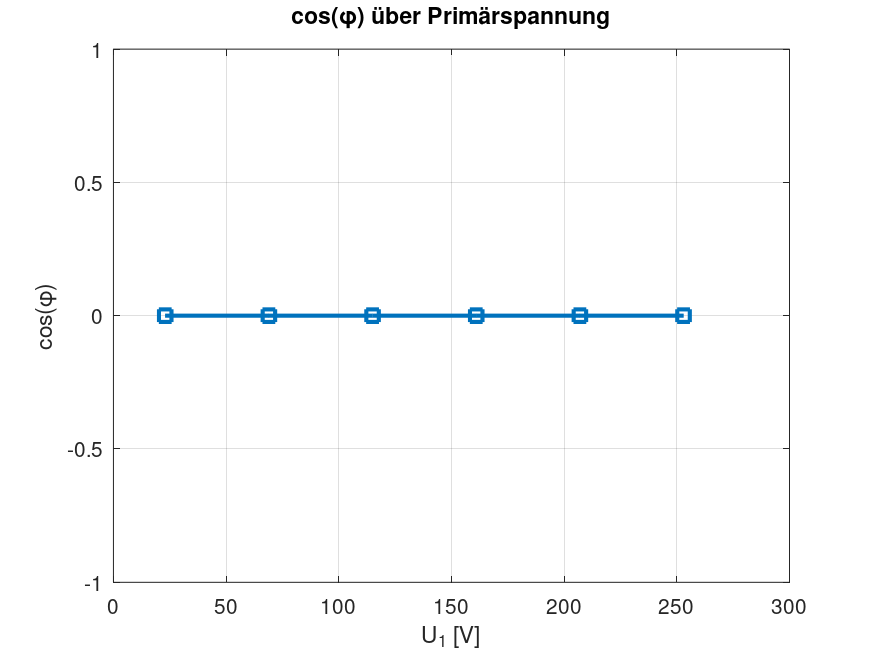
\includegraphics[width=0.7\linewidth]{images/Vorb-1-2-Leerlauf-cosphi}
						\caption{Leistungsfaktor $cos(\varphi)$ über Leerlaufspannung}
						\label{fig:vorb-1-2-leerlauf-cosphi}
					\end{figure}
					
				Zur Validierung kann man die Berechnung von $S$ über die folgende Formel heranziehen:
				
				\[
				\underline{S} = \underline{U}^2 \cdot \underline{Y^*}
				\]
				
				Nimmt man für die Spannung $\underline{U}$ einen Phasenwinkel von $0^\circ$ an, so ergibt sich der negative Phasenwinkel der Admittanz direkt als Winkel der Scheinleistung bzw. als Winkel des Leistungsfaktors.
				
				Aus den vorherigen Betrachtungen folgt für die Admittanz näherungsweise ein Winkel von etwa $-90^\circ$. Dies entspricht einem Leistungsfaktor von
				
				\[
				\cos(\varphi) \approx 0
				\]
				
				Da sich die Admittanz bei Änderungen der Spannungsamplitude nicht verändert, bleibt auch der Leistungsfaktor $\cos(\varphi)$ für alle Messpunkte konstant. Die Simulationswerte sind daher plausibel.
					
				
					
					
			\subsection{Simulation des Kurzschlusses}
			
				Im Simulationsmodell wird nun ein Sekundärseitiger Kurzschluss hergestellt. Die Spannung auf der Primärseite $U_{1k}$ des Transformators wird langsam erhöht, bis der Kurzschlussstrom $I_{1k}$ ca. $100mA$ beträgt.\\
				Anschließend wird in $100mA$ Schritten bis $1A$ erhöht.
				\begin{figure}[H]
					\centering
					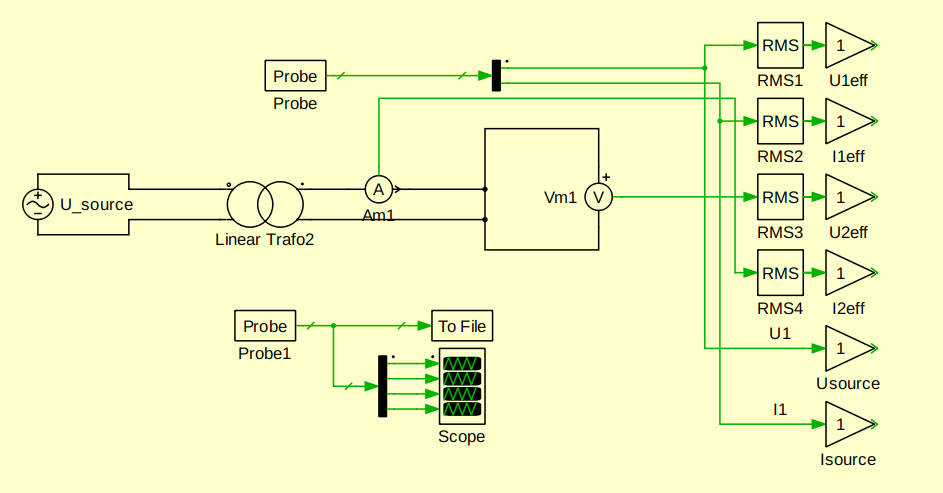
\includegraphics[width=\textwidth]{images/Vorb-1-3.png}
					\caption{Messaufbau der Kurzschlusssimulation in PLECS}
				\end{figure}
				
				Da $R_{Fe}$ laut Angabe unendlich groß wird, ist es durch die elektrische Parallelschaltung zu vernachlässigen. Das selbe gilt für $X_k$, welches ebenfalls elektrisch parallel geschalten wird.\newline
				\newline
				Das Ersatzschaltbild des Transformators im Kurzschlussfall lässt sich gemäß Abbildung~\ref{circ: ESBkurzschluss} darstellen.
				\begin{figure}[H]
					\centering
					\begin{circuitikz}
						% Spannungsquelle links
						\draw (0,0) to[sV, l=$U_{1k}$] (0,3)
						
						% Serienzweig: R1 und L1σ mit Strompfeil I10
						to[R, l=$R_k$, i=$I_{1k}$] (3,3)
						to[L, l=$X_{k}$] (6,3)
						
						% Ecke in der Rückleitung
						to(6,0)
						
						% Rückleitung
						-- (0,0);
						
					\end{circuitikz}
					\caption{Ersatzschaltbild des Transformators im Kurzschlussfall}
					\label{circ: ESBkurzschluss}
				\end{figure}
				
				Die Werte lassen sich wie folgt berechnen:
				
				\begin{formel}[H]
					\begin{align*}
						R_2' &= R2 \cdot "u^2 \\
						R_k &= R_1 + R_2' \\
						X_k &= X_{1\sigma} + X_{2\sigma}' = \sqrt{Z_k^2 - R_k^2} = \frac{U_{1}}{\sqrt{3} \cdot I_\mu} &mit \\
						I_\mu &= I_1 + \frac{I_2}{"u}
					\end{align*}
					\caption{Formeln zur Berechnung der Impedanzen im Kurzschlussfall}
				\end{formel}
				
				Daraus ergeben sich folgende simulierte Messwerte:
				\begin{table}[H]
					\begin{tabular}{c|c|c|c|c|c|c|c|c|c|c}
						$U_{1k}$ in V&  9.4 & 18.8 & 28.2 & 37.6 & 47 & 56.4 & 65.8 & 75.2 & 84.6 & 94\\
						$I_{1k}$ in A& 0.1 & 0.2 & 0.3 & 0.4 & 0.5 & 0.6 & 0.7 & 0.8 & 0.9 & 1.0\\
					\end{tabular}
					\caption{Messergebnisse aus Simulation des Kurzschlussfalls}
					\label{tab:Kurzschluss}
				\end{table}
				
				Aus den Messwerten ist ein linearer Zusammenhang zwischen der Kurzschlussspannung $U_{1k}$ und dem Kurzschlussstrom $I_{1k}$ erkennbar. Dies deutet darauf hin, dass die Kurzschlussimpedanz $Z_k$ des Transformators konstant ist.\newline
				\newline
				Für die Impedanz ergibt sich beispielsweise:
				\begin{formel}[H]
					$$
					Z_k = \frac{U_{1k}}{I_{1k}} \approx \frac{94,V}{1.0,A} = 94,\Omega
					$$
					\caption{Impedanz im Kurzschlussfall}
				\end{formel}
				Das lineare Verhalten bestätigt die Annahme des vereinfachten Ersatzschaltbildes, bei dem der Magnetisierungszweig vernachlässigt wird. Der Transformator wird im Kurzschlussfall somit im Wesentlichen durch die Serienimpedanz bestehend aus Kupferwiderständen und Streureaktanzen beschrieben. \newline
				\newline
				Nichtlineare Effekte, wie beispielsweise die Reaktanz $X_h$ des Transformators als Induktivität, sind im betrachteten Bereich nicht erkennbar.
				
				\subsubsection{Effektivwert des Kurzschlussstroms $I_{1k}$ über Effektivwert der Primärspannung $U_{1k}$}
					\begin{figure}[H]
						\centering
						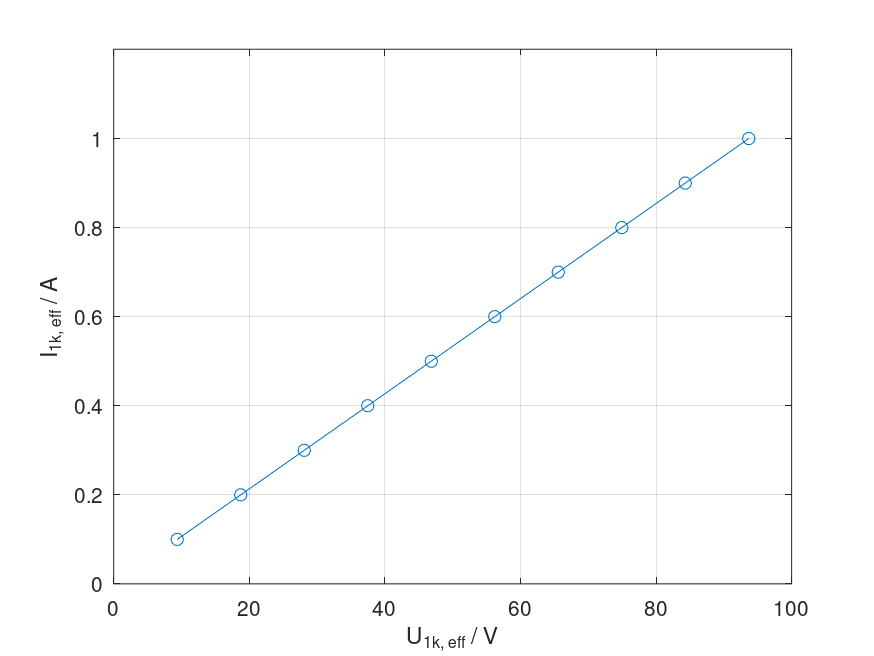
\includegraphics[width=\textwidth]{images/Vorb-1-3-Kurzschluss_I1-U1.png}
						\caption{Effektivwert des Kurzschlussstroms $I_{1k}$ über Effektivwert der Primärspannung $U_{1k}$}
					\end{figure}
					Der dargestellte Verlauf zeigt einen linearen Zusammenhang zwischen dem Kurzschlussstrom $I_{1k}$ und der angelegten Primärspannung $U_{1k}$. Dies bestätigt, dass sich der Transformator im Kurzschlussfall wie eine lineare Impedanz verhält.\newline
					\newline
					Die Steigung der Kennlinie entspricht dabei dem Kehrwert der Kurzschlussimpedanz:
					\begin{formel}
						$$
							\frac{\Delta I_{1k}}{\Delta U_{1k}} = \frac{1}{Z_k}	
						$$
						\caption{Zusammenhang des Kurzschlussstroms und der Primärspannung}
					\end{formel}
					
					Da die Kennlinie eine Gerade durch den Ursprung darstellt, kann von einer konstanten Impedanz $Z_k$ ausgegangen werden. Dies stimmt mit dem vereinfachten Ersatzschaltbild überein, bei dem lediglich die Serienimpedanz aus Kupferwiderständen und Streureaktanzen berücksichtigt wird.\newline
					\newline
					Nichtlineare Effekte, insbesondere eine magnetische Sättigung des Kerns, treten im betrachteten Bereich nicht auf, da die angelegte Spannung vergleichsweise gering ist.
					
				\subsubsection{Effektivwert des Kurzschlussstroms $I_{2k}$ über Effektivwert der Primärspannung $U_{1k}$}
					\begin{figure}[H]
						\centering
						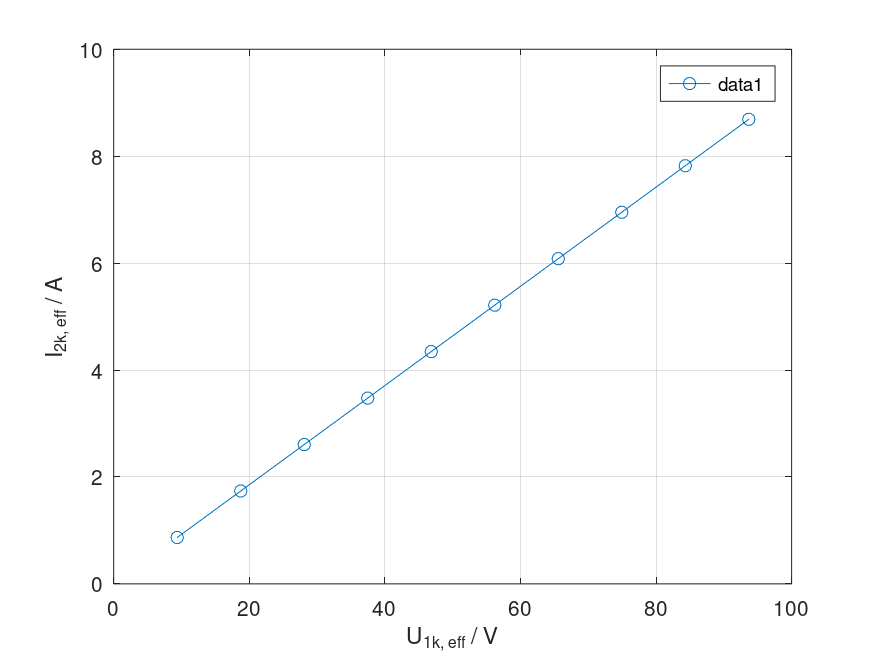
\includegraphics[width=\textwidth]{images/Vorb-1-3-Kurzschluss_I2-U1.png}
						\caption{Effektivwert des Kurzschlussstroms $I_{2k}$ über Effektivwert der Primärspannung $U_{1k}$}
					\end{figure}
					Der Verlauf des Kurzschlussstroms $I_{2k}$ in Abhängigkeit von der Primärspannung $U_{1k}$ zeigt ebenfalls einen linearen Zusammenhang. Dies ist zu erwarten, da der Sekundärstrom über das Übersetzungsverhältnis direkt mit dem Primärstrom gekoppelt ist.\newline
					\newline
					Für den idealen Transformator gilt:
					\begin{formel}
						$$
							I_{2k} = "u \cdot I_{1k}
						$$	
						\caption{Abhängigkeit des Sekundären Kurzschlussstroms über des Primären Kurzschlussstroms und dem Windungsfaktor}
					\end{formel}
					
					Da bereits für den Primärstrom ein linearer Zusammenhang mit der Spannung festgestellt wurde, ergibt sich auch für den Sekundärstrom eine proportionale Abhängigkeit von der Primärspannung.\newline
					Die lineare Kennlinie bestätigt somit, dass das Transformatorverhalten im Kurzschlussfall durch die konstante Serienimpedanz bestimmt wird.
					
				\subsubsection{Leistungsfaktor $cos \varphi_k$ im Kurzschluss über Effektivwert der Primärspannung $U_{1k}$}
					\begin{figure}[H]
						\centering
						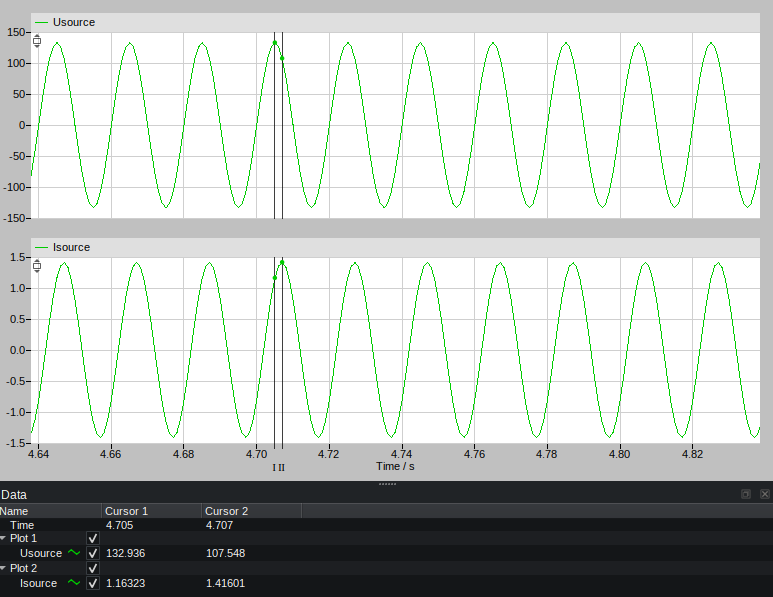
\includegraphics[width=\textwidth]{images/Vorb-1-3-Kurzschluss-Leistungsfaktor.png}
						\caption{Leistungsfaktor $cos \varphi_k$ im Kurzschluss über Effektivwert der Primärspannung $U_{1k}$}
					\end{figure}
					Bei näherer Betrachtung ergibt $\Delta t$ einen Wert von 0.002s.\\
					Daraus folgt:
					\begin{formel}
						\begin{align*}
							\varphi_{UI} &= 360 \cdot 50Hz \cdot 0.002s = 36\degree	\\
						\end{align*}
						\caption{Berechnung von $\varphi$ im Kurzschlussfall}
					\end{formel}

					Der Verlauf des Leistungsfaktors $\cos(\varphi_k)$ zeigt über den betrachteten Bereich konstante Werte. Dies lässt sich dadurch erklären, dass sich das Verhältnis von Wirk- zu Blindanteil der Impedanz im Kurzschlussfall nicht ändert.\newline
					\newline
					Die Kurzschlussimpedanz $Z_k$ setzt sich aus dem ohmschen Widerstand $R_k$ und der induktiven Reaktanz $X_k$ zusammen:
					\begin{formel}
						$$
							Z_k = R_k + j X_k	
						$$
						\caption{Zusammensetzung von $R_k$ und $X_k$ im Kurzschlussfall}
					\end{formel}

					Da beide Größen als auch die Frequenz konstant sind, bleibt auch der Phasenwinkel $\varphi_k$ zwischen Strom und Spannung unverändert. Folglich ergibt sich ein konstanter Leistungsfaktor.\newline
					\newline
					Der zuvor bestimmte Phasenwinkel von etwa $\varphi \approx 36^\circ$ führt zu einem Leistungsfaktor $\lambda$ von
					\begin{formel}
						$$
							\lambda = \cos(\varphi_k) \approx 0{,}81
						$$
						\caption{Leistungsfaktor im Kurzschlussfall}
					\end{formel}
					
					Dies bestätigt, dass im Kurzschlussfall sowohl ohmsche als auch induktive Anteile zur Impedanz beitragen und das Verhalten des Transformators durch eine feste komplexe Impedanz beschrieben werden kann.
					
			\subsection{Simulation des Einschaltstroms (Eng.: inrush current)}
				
			\begin{figure}[H]
				\centering
				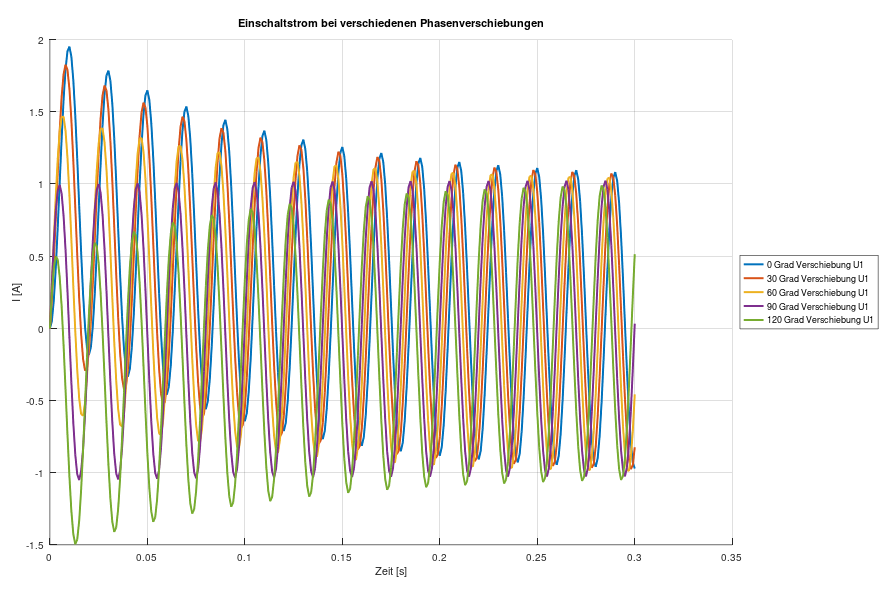
\includegraphics[width=1\linewidth]{images/Vorb-1-4-einschaltstrom}
				\caption{Einschaltstrom I1 bei verschiedenen Phasenlagen von U}
				\label{fig:vorb-1-4-einschaltstrom}
			\end{figure}
			 
	
				
	\section{Versuchsdurchführung}
		Der Transformator hat 3 getrennte Wicklungssätze mit jeweils 3 Wicklungen pro Wicklungssatz. Diese werden Primär-, Sekundär- und Tertiäre Wicklung bezeichnet.
		\begin{center}
			1U1 - 1U2, 1V1 - 1V2, 1W1 - 1W2\\
			2U1 - 2U2, 2V1 - 2V2, 2W1 - 2W2\\
			3U1 - 3U2, 3V1 - 3V2, 3W1 - 3W2
		\end{center} 
		Für diese Versuchsreihe wird eine Reihenschaltung mit der Wicklung 2U1 - 2U2 und 3U1 - 3U2 gebildet. Die Spannungsversorgung wird mittels Leiter-Leiter-Spannung Primärseitig an 1U1 - 1U2 angesetzt. Dadurch kann der Transformator einphasig betrieben werden.
		
		\subsection{Typenschild und Nennwerte des Transformators}
		
			\begin{table}[H]
				\begin{tabular}{l l l}
					\hline \\
					Bgr: DUSTA8095 & Nr.: 011182 & kVA: 20000 \\
					prim: 400V & A: 31 & Hz: 50/60 \\
					sec.: 110/110V & A: 52,5/52,5 & nach VDE: 0550 \\
												& & Iso. Klasse: T40F \\
					\hline
				\end{tabular}
				\caption{Typenschild des einphasigen Transformators}
			\end{table}
			Die angegebene Spannung beschreibt immer Leiter-Leiter-Spannung
			Herkömmliche Transformatoren weisen auf ihre interne Beschaltung am Typenschild hin. Diesem ist sie jedoch dem Aufgabenblatt zu entnehmen:
			\begin{center}
				Primärseite in Dreieckschaltung\\
				Sekundärseite in Sternschaltung\\
				Tertiärseite in Sternschaltung		
			\end{center}
			
			Aus dem Datenblatt und der Erkenntnis interner Beschaltungen lassen sich Nennspannung und Nennstrom des einphasigen Transformators berechnen.
			\begin{formel}
				\begin{align*}
					U_{N, Str} &= \frac{400V}{\sqrt{3}} = 231V \\
					I_{N, Str} &= \frac{31}{\sqrt{3}} = 17,9A
				\end{align*}	
				\caption{$U_{N1}$ und $I_{N1}$}
			\end{formel}
			
			\begin{formel}
				\begin{align*}

				\end{align*}	
				\caption{$U_{N2}$ und $I_{N2}$}
			\end{formel}
			
			\begin{formel}
				\begin{align*}
					U_{N3} &= U_{N2} \\
					I_{N3} &= I_{N3}
				\end{align*}	
				\caption{$U_{N3}$ und $I_{N3}$}
			\end{formel}
			
			
>>>>>>> 12ac912d5f0cd10c8a41cde0f36251f4203ee1ef
	\section{Versuchsauswertung}
	
	\section{Checkliste für die Versuchsausarbeitung}
	%\begin{figure}[H]
	%	\centering
	%	\includegraphics{HIER DIE CHECKLISTE EINFÜGEN}
	%\end{figure}
	
	\newpage
	\printbibliography % WIRD ANGEZEIGT WENN BIB VERWENDET WIRD
\end{document}